\section{Introduction}
\label{sec:intro}

Some properties of natural and engineered materials can be analyzed  by
treating them as stacked two dimensional (2D) layers.
The structure within each layer could be
self-similar \cite{Intro1}
spanning multiple scales,
generally aperiodic and quasi-uniform within any one scale,
and consisting of a few repeated motifs appearing in disordered
arrangements. Each layer is not necessarily planar, i.e.,
it consists of multiple,
inter-constraining planar (genus 0) monolayers.
Furthermore, a layer is often  either
{\sl isostatic or underconstrained, not
self-stressed} (See Section \ref{sec:prelim} for definitions).
These properties are
consistent with a self-assembled 2D structure that minimizes mass,
optimally distributes external stresses and itself
participates in the assembly of diverse and multifunctional,
larger 2D structures.

Examples of such materials (See Figure \ref{examples}) include:

\begin{figure*}\centering
\begin{subfigure}{.31\linewidth}\centering
  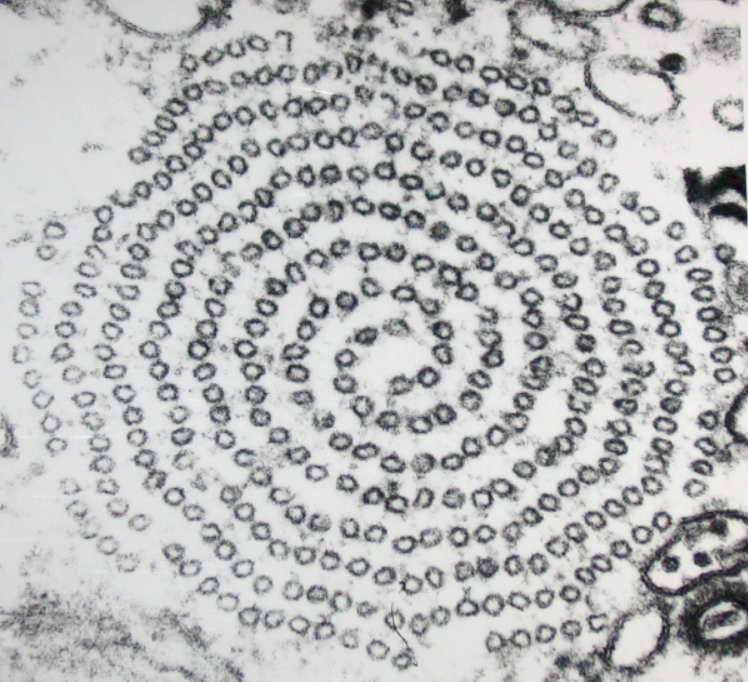
\includegraphics[width=\linewidth]{img/Axopodium_Mikrotubuli}
  \caption{Cross section of a Heliozoa's psuedopod, formed by a spiral structure of microtubules.}
  % https://de.wikipedia.org/wiki/Mikrotubulus#mediaviewer/File:Axopodium_Mikrotubuli.jpg
  \label{fig:microtubule}
\end{subfigure}\hfill
\begin{subfigure}{.31\linewidth}\centering
  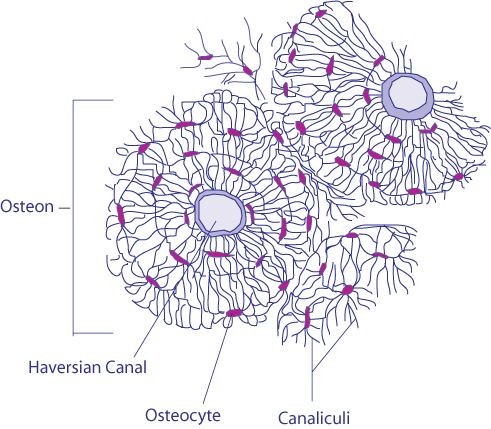
\includegraphics[width=\linewidth]{img/Transverse_Section_Of_Bone}
  \caption{Cross section of an osteon (the fundamental unit of compact bone) exhibiting its hierarchical structure.}
  % https://en.wikipedia.org/wiki/Osteon#mediaviewer/File:Transverse_Section_Of_Bone.png
  \label{fig:osteon}
\end{subfigure}\hfill
\begin{subfigure}{.31\linewidth}\centering
  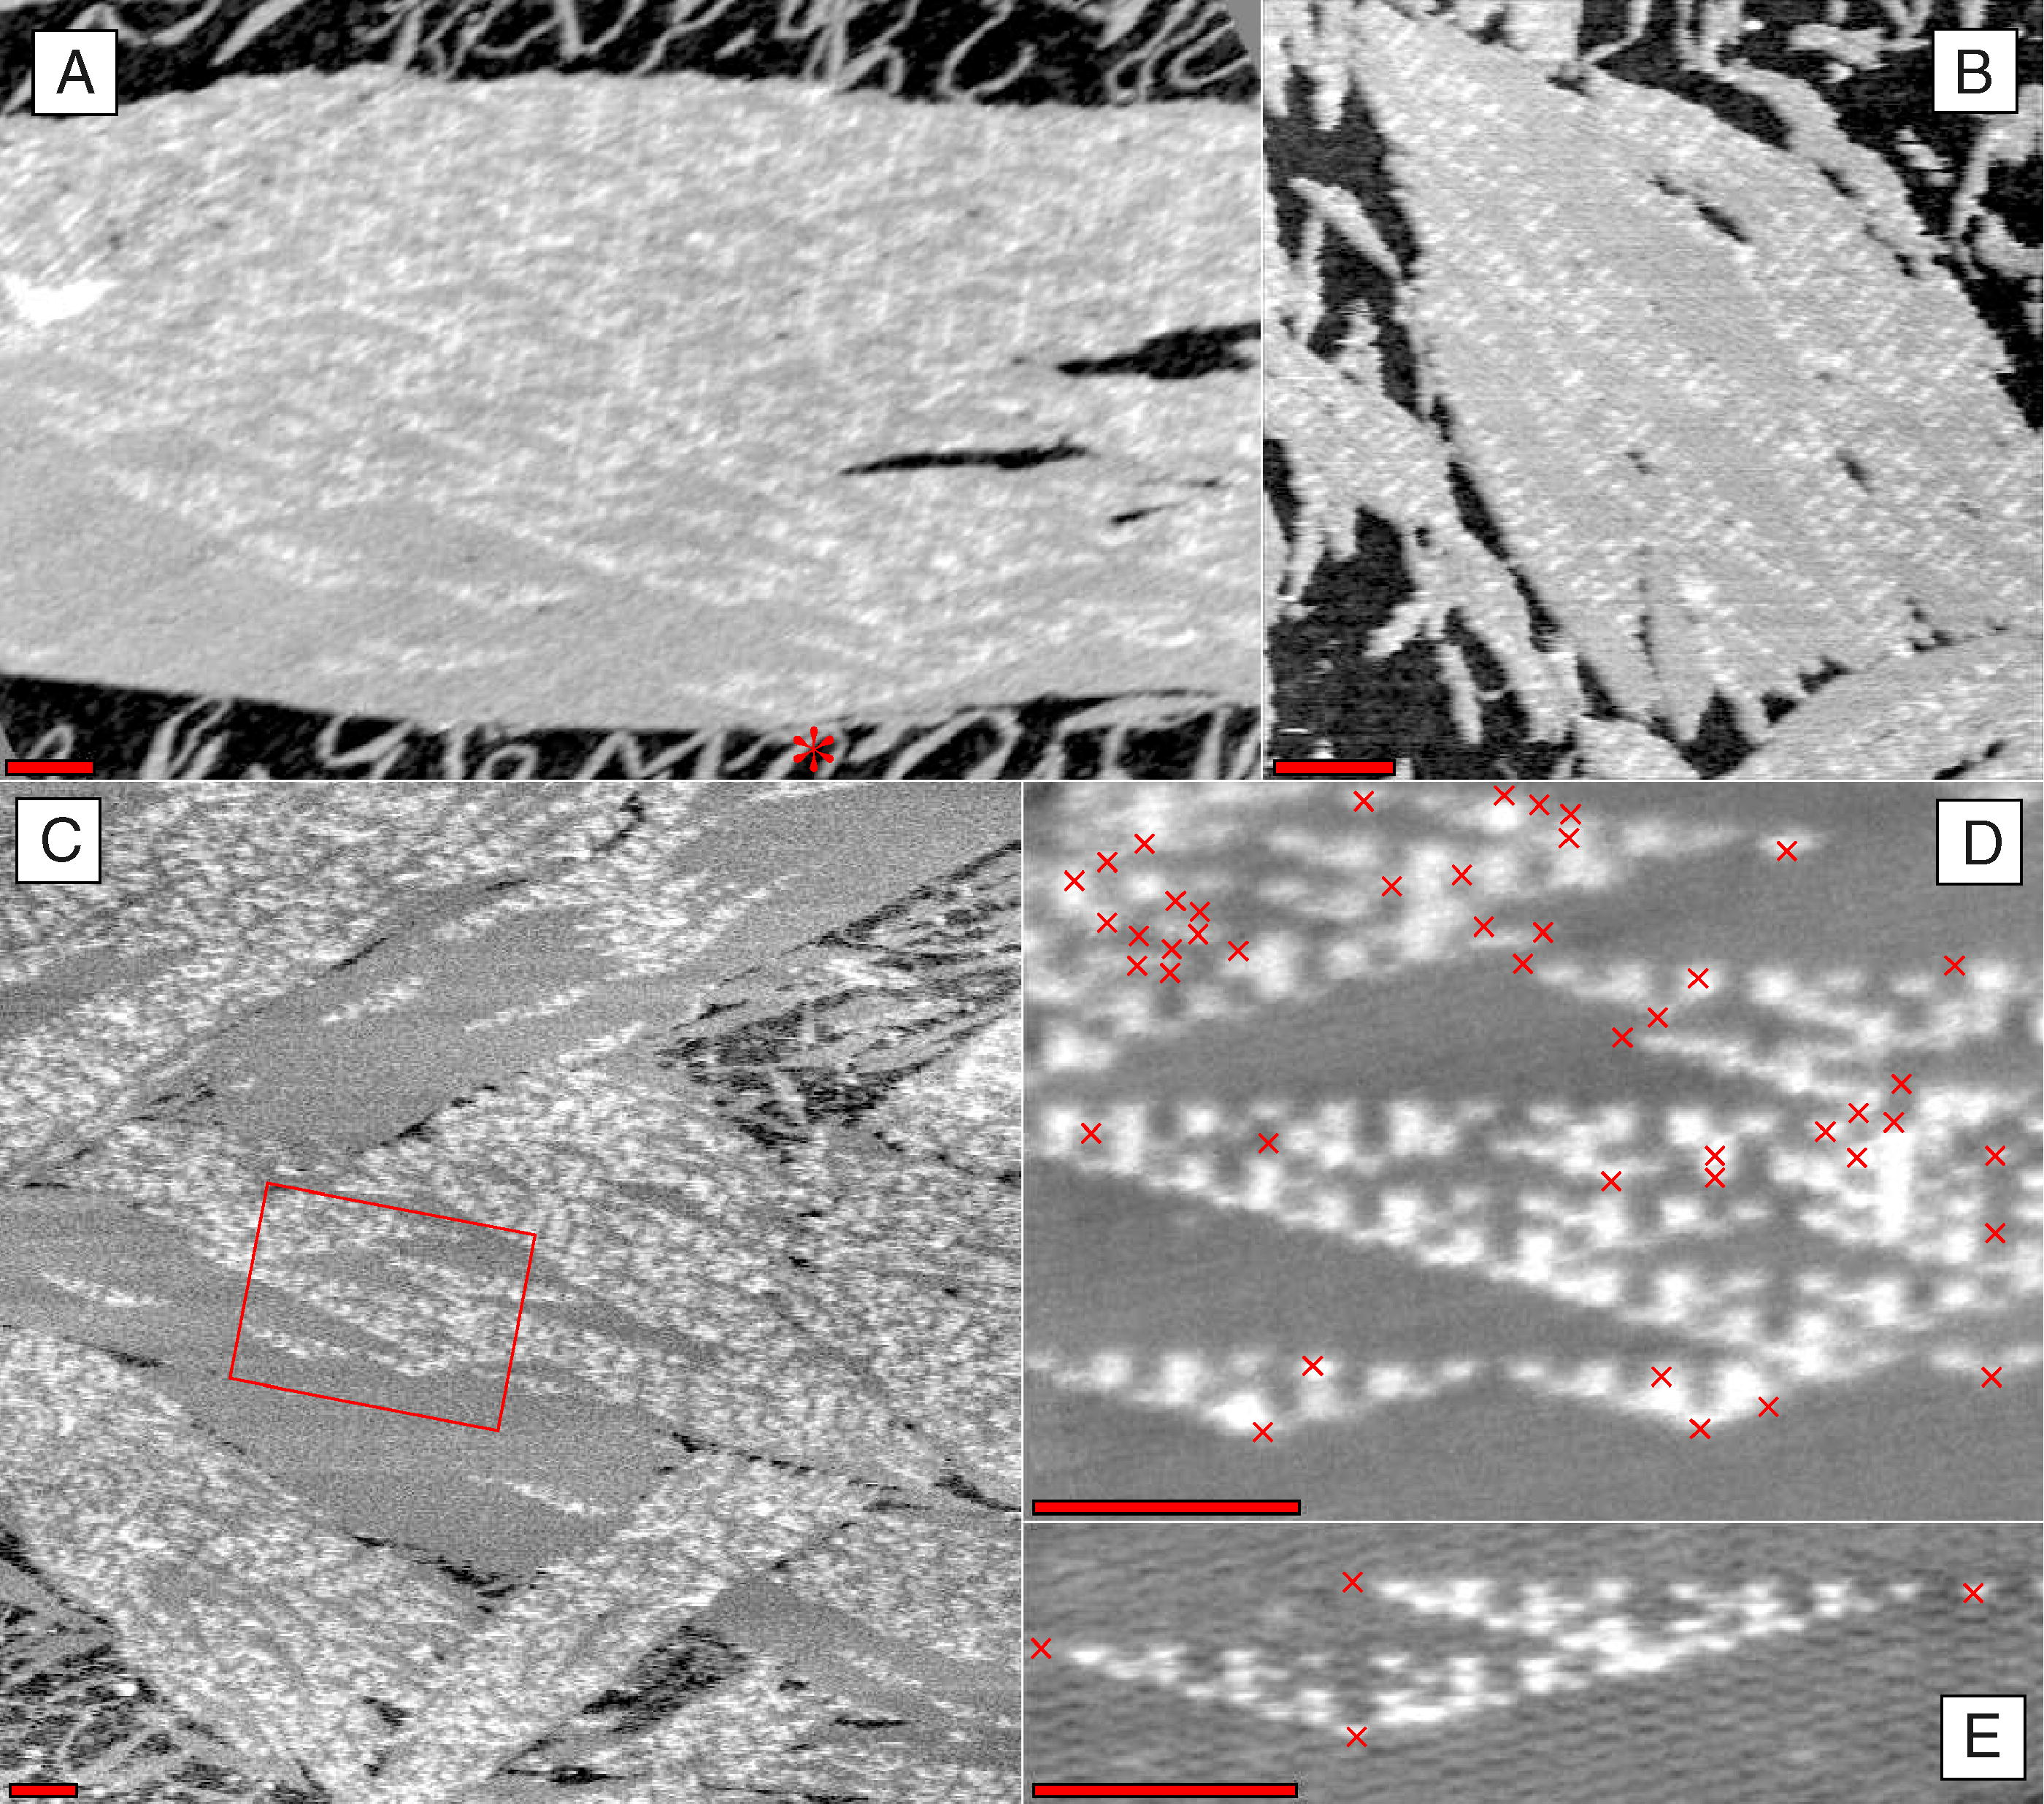
\includegraphics[width=\linewidth]{img/Rothemund-DNA-SierpinskiGasket}
  \caption{A DNA array exhibiting the Sierpinski triangle.}
  % https://en.wikipedia.org/wiki/DNA_nanotechnology#mediaviewer/File:Rothemund-DNA-SierpinskiGasket.jpg
  \label{fig:sierpinski}
\end{subfigure}
\caption{}
\end{figure*}


\begin{enumerate}
  %
    \item (cross-section) of microtubules \cite{Necklace1} e.g., in
ciliary membranes and transitions \cite{Necklace2}
   %
    \item (cross-section) of hierarchical bone structure \cite{XX} %
    \item crosslinked cellulose or collagen microfibril monolayers e.g.,
in cell-walls \cite{CellWalls1} \cite{CellWalls1}, as well as crosslinked
actin filaments in the cytoskeleton matrix.
  %
    \item more recent, engineered examples including  disordered graphene
layers \cite{Graphene1} \cite{Graphene2} sometimes reinforced
    by  microfibrils; and DNA assemblies \cite{Microfibrils1} including a
recent Sierpinski carpet, bringing other self-similar structures
    \cite{Microfibrils2} within reach.
    %
    \item  silica bi-layers, glass \cite{SilicaGlass1}
\cite{SilicaGlass2}, and materials that behave like assemblies of
    2D particles under non-overlap constraints, e.g, jammed
    disks on the plane \cite{JammedDisk1}
%
\end{enumerate}
%
In order to study structural and mechanical properties
such as rigidity, flexes and distribution of external stresses
within the material layer, it is natural to model a material
layer as a solution of a geometric constraint system
of appropriate types of geometric primitives, under
metric or algebraic constraints.
Such  2D {\bf{\em qusecs}} (quasi-uniform or self-similar
constraint systems) can be used to
understand or design material layers (their solutions)
with desired properties.
%
\subsection{Previous Work on Relevant 2D Geometric Constraint Systems} We
now briefly survey existing techniques for studying 2D {\em qusecs,}  many
of which are {\it bar-joint} systems (Examples 1,2 above, see Sections
\ref{sec:DRP}, \ref{sec:recomb}),
{\it multibody-pin} systems (Example 4,5, see Section \ref{sec:bodypin}) or  {\it
pinned-line incidence} systems (Example 3, see Section \ref{sec:pinnedline}). The
limitations of these techniques directly motivate
the contributions of this paper.

\medskip\noindent\underbar{{\sl (i) Finding (vertex)-maximal
generically rigid subsystems}}
Fast, graph-based algorithms exist (pebble-game \cite{XX}),
for locating all maximal, generically rigid subsystems \cite{XX}.
When the input is rigid, these algorithms compute the identity and  output
the input.

However, both for self-similar or just aperiodic 2D qusecs, it is
imperative to recursively decompose rigid systems
into their rigid subsystems, down to the level of
geometric primitives, in order to
understand or design properties at all scales, such as:
rigidity, flexes, distribution
of external stresses, boundary conditions for isostaticity,
as well as behavior under constraint variations.

\medskip\noindent\underbar{{\sl (ii) Optimal Recursive Decomposition
(DR-planning)}}
Recursive decomposition of geometric constraint systems has been
formalized \cite{XX} and well-studied \cite{XX}
as the {\sl Decomposition-Recombination (DR)-planning} problem.
For the above-mentioned classes of 2D qusecs, generic rigidity is
a combinatorial property and hence each level of the decomposition should,
in principle, be achievable by a graph-based algorithm as in (1), without
involving geometric information in the constraint system.
Since many  such decompositions can exist for a given constraint system,
criteria defining desirable or optimal DR-plans and DR-planning algorithms
were given in \cite{XX}. An {\em optimal DR-plan} is one
that minimizes the maximum number of child subsystems of any parent
system, a property that is
crucial for obtaining a solution to the parent constraint system from the
solutions of the child systems.

However, for general 2D qusecs, even when restricted to bar-joint systems,
the optimal DR-planning problem was shown to be NP-hard \cite{XX}.

\medskip\noindent\underbar{{\sl (iii) DR-plans for special classes and
with other criteria}}
For a special class of 2D qusecs, namely  {\em tree-decomposable} systems
\cite{XX} common in computer aided mechanical design,
(which includes ruler-and-compass and Henneberg-I constructible systems),
all DR-plans turn out to
be optimal. This satisfies the so-called {\em Church-Rosser} criterion,
leading to highly efficient DR-planning algorithms.
For general 2D qusecs, alternate criteria were suggested
such as {\em cluster minimality}
requiring parent systems to be composed of
a minimal set of at least 2 rigid proper subsystems (i.e., no proper
subset forms a rigid system);
and {\em proper maximality}, requiring child subsystems
to be maximal rigid proper subsystems of the parent system.

While polynomial time algorithms were given \cite{XX} to generate DR-plans
meeting the cluster minimality criterion,
no such algorithm is known for the latter criterion.


\medskip\noindent\underbar{{\sl (iv) Optimal Recombination and Solution
Space Navigation}}
For the entire DR-plan, finding all
desired solutions is barely tractable even if recombination
of solved subsystems is easy for each indecomposable parent system in the
DR-plan.
This is because even for the simplest, highly decomposable systems
with small DR-plans, the problem of finding even a single
solution to the input system at the root of the DR-plan
is NP-hard \cite{XX} and there is a
combinatorial explosion of solutions \cite{XX}. Typically, however,
the desired solution has a given orientation type, in which case,
the crux of the difficulty is concentrated in the algebraic complexity of
(re)combining child system solutions, to give a
solution to the parent system at any
given level of the DR-plan.
For fairly general 3D constraint systems,
there are algorithms with formal
guarantees that uncover underlying matroids to combinatorially
obtain an optimal parameterization to minimize the algebraic
complexity of the indecomposable parent (sub)systems that occur in the
DR-plan \cite{XX, XX,XX},
provided the DR-plan meets some of the abovementioned criteria.

However, the generality of these algorithms
trades-off against efficiency, and despite the optimization,
the best algorithms can still take
exponential time in the number of child subsystems (which can be arbitrarily
large even for optimal DR-plans) in order to guarantee
all solutions of a given orientation type,
even for a single (sub)system in a DR-plan. They
are prohibitively slow in practice. We note that utilizing the DR-plan and
optimal recombination as a principled basis, high performance heuristics
and software
exists \cite{XX,XX} to
tame combinatorial explosion via user intervention.


\medskip\noindent\underbar{{\sl (v) Configuration Spaces of
Underconstrained Systems}}
For underconstrained 2D bar-joint and multibody-pin cusecs obtained from
various subclasses of tree-decomposable systems, algorithms have been
developed \cite{XX, XX} that
to complete them into isostatic systems \cite{XX, XX} and to find paths
within the connected components \cite{XX,XX} of
standard cartesian configuration spaces. Most of the algorithms with
formal guarantees leverage Cayley configuration space theory \cite{XX,XX}
to characterize subclasses of graphs and additional constraints that
control combinatorial explosion, and provide faithful bijective
representation
of connected components and paths.
These algorithms have decreasing efficiency as the subclass of systems
gets bigger,  with highest efficiency for
underlying partial 2-tree graphs (alternately, tree-width 2,
series-parallel, $K_4$ minor avoiding),   moderate efficiency for
1 degree-of-freedom (dof) graphs with low Cayley complexity (which include
common linkages such as the Strandbeest, Limacon and Cardioid), and
decreased efficiency for general 1-dof tree-decomposable graphs. While
software suites exist \cite{XX,XX}, no such formal algorithms and
guarantees are known for non-tree-decomposable systems.
%
\subsection{Contributions and Organization}
\label{sec:cont}
The contributions of this paper are the following.
\begin{itemize}
\item
We  navigate the NP-hardness barrier mentioned in (2) above, for finding
optimal DR-plans by defining a
so-called {\it canonical} DR-plan and showing a strong Church-Rosser
property: {\it all canonical DR-plans for isostatic or
underconstrained
2D qusecs are optimal} (Section \ref{sec:DRP}).
\item
We give an efficient ($O(n^2)$) algorithm to find a canonical (and hence
optimal) DR-plan for all 3 types of 2D qusecs mentioned above (Sections
\ref{sec:DRP}, \ref{sec:bodypin}, and \ref{sec:pinnedline}.
The canonical DR-plan
illuminates the essence of the NP-hardness of finding optimal DR-plans for
overconstrained systems.
\item
We give a method to deal with the
algebraic complexity of recombining the realizations or
solutions of  child subsystems into a solution of the parent system.
Specifically, we define the problem of  minimally modifying the
indecomposable recombination system so that it becomes decomposable via a
 small DR-plan and yet preserves the original
solutions in an efficiently searchable manner. We show formal connection
to well known problems such as optimal completion of
underconstrained  systems  \cite{XX}.  When the required modifications
are bounded, we obtain new, efficient algorithms for
realizing both isostatic and underconstrained
qusecs by leveraging recent results about Cayley parameters in
\cite{XX,XX}  (Section \ref{sec:recomb}).
\item
We briefly describe applications of the above techniques to modeling,
analyzing and designing specific properties in 2D material layers.
For Examples 1,2 (achieving isostaticity, distribution of stresses in
self-similar, bar-joint systems); Example 3 (canonical and optimal
DR-plans for pinned line incidence systems \cite{XX}) and Examples 4,5
(boundary-conditions for achieving various desired properties
of multi-body  pin systems).

\item
Software implementation and videos can be found at: \todo{Provide Link}.
\end{itemize}
